% BEGIN LICENSE BLOCK
% Version: CMPL 1.1
%
% The contents of this file are subject to the Cisco-style Mozilla Public
% License Version 1.1 (the "License"); you may not use this file except
% in compliance with the License.  You may obtain a copy of the License
% at www.eclipse-clp.org/license.
% 
% Software distributed under the License is distributed on an "AS IS"
% basis, WITHOUT WARRANTY OF ANY KIND, either express or implied.  See
% the License for the specific language governing rights and limitations
% under the License. 
% 
% The Original Code is  The ECLiPSe Constraint Logic Programming System. 
% The Initial Developer of the Original Code is  Cisco Systems, Inc. 
% Portions created by the Initial Developer are
% Copyright (C) 2006 Cisco Systems, Inc.  All Rights Reserved.
% 
% Contributor(s): 
% 
% END LICENSE BLOCK
%
% $Id: umsusing.tex,v 1.2 2009/07/16 09:11:24 jschimpf Exp $
%
% Imported from the user manual


\newcommand{\guitext}[1]{\mbox{\texttt{#1}}}
\newcommand{\keyboard}[1]{{\texttt{#1}}}
%\newcommand{\menu}[1]{{\texttt{#1}}}
%\newcommand{\menuopt}[1]{{\texttt{#1}}}
%\newcommand{\button}[1]{{\texttt{#1}}}
\newcommand{\menu}[1]{\guitext{#1}}
\newcommand{\menuopt}[1]{\guitext{#1}}
\newcommand{\button}[1]{\guitext{#1}}

\newcommand{\ignore}[1]{}

%------------------------------------------------------------------------
\chapter{Getting started with {\eclipse}}
%------------------------------------------------------------------------
\label{chapusing}
%HEVEA\cutdef[1]{section}

%------------------------------------------------------------------------
\section{How do I install the {\eclipse} system?}
%------------------------------------------------------------------------
Please see the installation notes that came with {\eclipse}.
For Unix/Linux systems, these are in the file \texttt{README_UNIX}.
For Mac~OS~X, they are in the file \texttt{README_MACOSX}.

For Windows, the installation process is usually via an automatic
installer. Instructions for manual installation can be found in
\texttt{README_WIN.TXT}.

Please note that choices made at installation time can affect which
options are available in the installed system.

%------------------------------------------------------------------------
\section{How do I read the online documentation?}
%------------------------------------------------------------------------
Under Unix and Mac~OS~X, use any HTML browser to open the file \verb+doc/index.html+
in the \eclipse{} installation directory.
Under Windows, select the menu entry
\begin{verbatim}
Start - Programs - ECLiPSe - Documentation
\end{verbatim}

%------------------------------------------------------------------------
\section{How do I run my {\eclipse} programs?}
%------------------------------------------------------------------------
There are two ways of running {\eclipse} programs.  The first is using
\texttt{tkeclipse}, which provides an interactive graphical user
interface to the {\eclipse} compiler and system.  The second is using
\texttt{eclipse}, which provides a more traditional command-line
interface.  We recommend you use {\tkeclipse} unless you have some
reason to prefer a command-line interface.

%------------------------------------------------------------------------
\section{How do I use \texttt{tkeclipse}?}
%------------------------------------------------------------------------

\subsection{Getting started}

To start {\tkeclipse}, either type the command \texttt{tkeclipse} at
an operating system command-line prompt, or select {\tkeclipse} from
the program menu on Windows.  This will bring up the {\tkeclipse}
top-level, which is shown in Figure~\ref{tktop}.

\begin{figure}[bt]
\begin{center}
% funny pathname because this chapter gets included from tutorial as well
\resizebox{0.6\textwidth}{!}{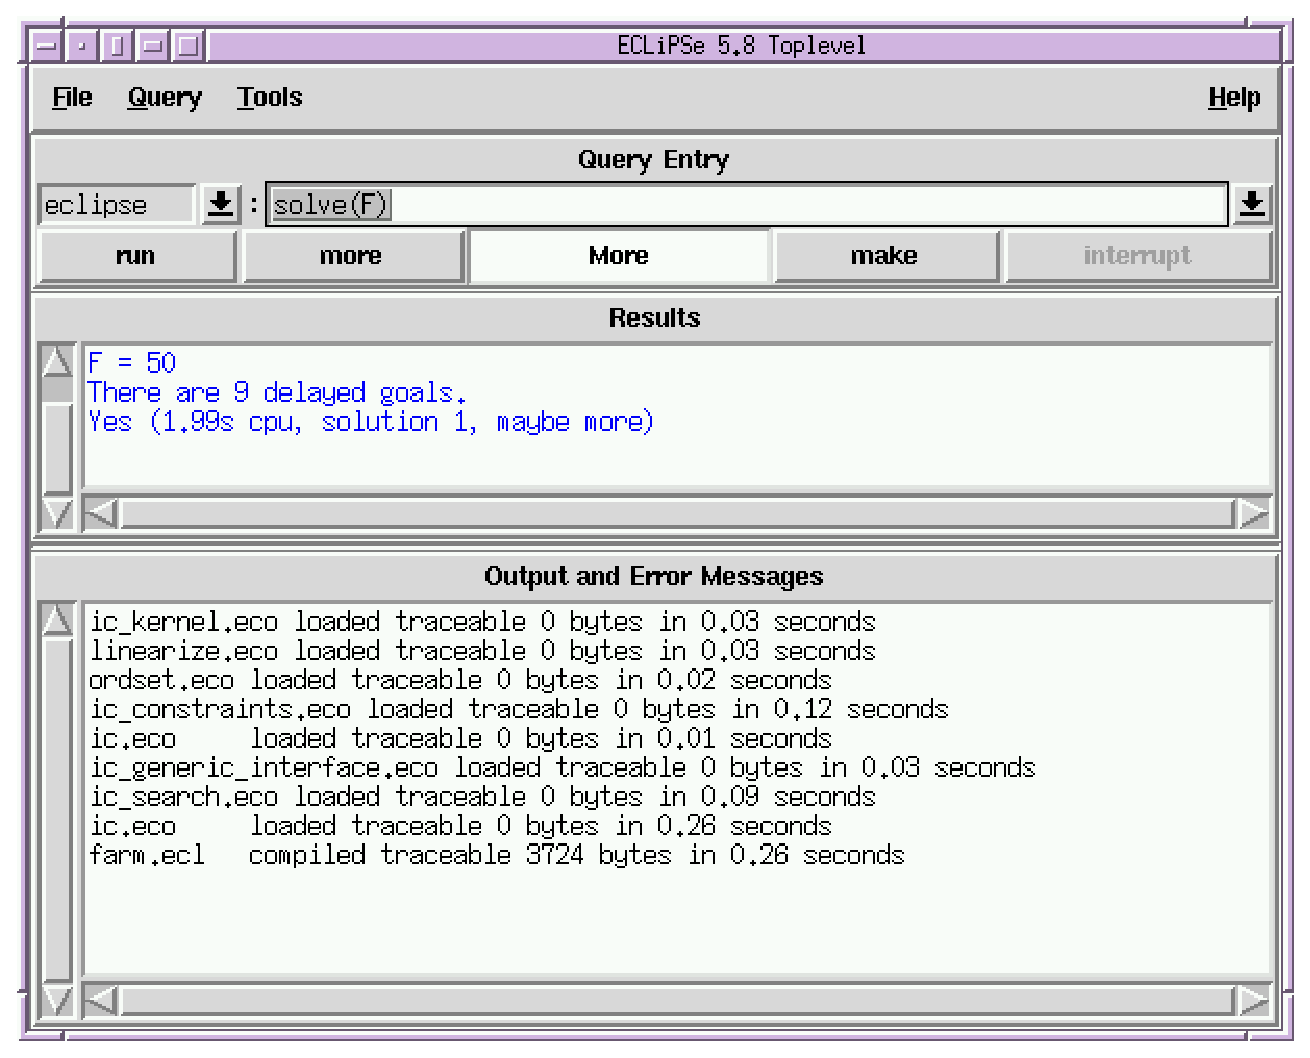
\includegraphics{../userman/tktop.eps}}
\end{center}
\caption{{\tkeclipse} top-level}
\label{tktop}
\end{figure}

Note that help on {\tkeclipse} and its component tools is available
from the \menu{Help} menu in the top-level window.

%------------------------------------------------------------------------
\section{How do I write an {\eclipse} program?}
%------------------------------------------------------------------------
You need to use an editor to write your programs. {\eclipse} does not come
with an editor, but any editor that can save plain text files can be used. 
Save your program as a plain text file, and you can then compile the
program into {\eclipse} and run it.

Extra support for editing {\eclipse} programs with common editors are
available. An eclipse mode for the GNU emacs editor is bundled with the
{\eclipse} package. This mode provides syntax highlighting, automatic
indentation and many other features. To use this mode, you need to load the
\texttt{eclipse.el} file into emacs. This is done by adding the following
line to your \texttt{.emacs} file:

\begin{small}
\begin{verbatim}
(autoload 'eclipse-mode "<eclipsedir>/lib_public/eclipse.el" "ECLIPSE editing mode" t)
\end{verbatim}
\end{small}

where \texttt{<eclipsedir>} is the path to your {\eclipse} installation
directory. 
 
With {\tkeclipse}, you can specify the editor you want to use, and this
editor will be started by {\tkeclipse}, e.g. when you select a file in
the `Edit' option under the File menu. The default values are the value of
the VISUAL environment variable  under Unix, or Wordpad under Windows.
This can be changed with the Preference Editor under the Tools menu.

%------------------------------------------------------------------------
\subsection{Compiling a program}

\index{compile}
From the \menu{File} menu, select the \menuopt{Compile ...} option.
This will bring up a file selection dialogue.  Select the file you wish
to compile, and click on the \button{Open} button.  This will compile
the file and any others it depends on.  Messages indicating which
files have been compiled and describing any errors encountered will be
displayed in the bottom portion of the {\tkeclipse} window
(\guitext{Output and Error Messages}).

If a file has been modified since it was compiled, it may be
recompiled by clicking on the \guitext{make} button.  This recompiles
any files which have become out-of-date.

\See{For more information on program compilation and the compiler,
please see \textbf{The Compiler} chapter in the user manual.}

%------------------------------------------------------------------------
\subsection{Executing a query}

\index{query}
To execute a query, first enter it into the \guitext{Query Entry} text
field.  You will also need to specify which module the query should be
run from, by selecting the appropriate entry from the drop-down list
to the left of the \guitext{Query Entry} field.  Normally, the default
selection of \guitext{eclipse} will be fine; this will allow access to
all {\eclipse} built-ins and all predicates that have not explicitly
been compiled into a different module.  Selecting another module for
the query is only needed if you wish to call a predicate which is not
visible from the {\tt eclipse} module, in which case you need to
select that module.  \See{For more information about the module
system, please see the \textbf{Module System} chapter in the user
manual.}

To actually execute the query, either hit the \keyboard{Enter} key
while editing the query, or click on the \guitext{run} button.
{\tkeclipse} maintains a history of commands entered during the
session, and these may be recalled either by using the drop-down list
to the right of the \guitext{Query Entry} field, or by using the up
and down arrow keys while editing the \guitext{Query Entry} field.

If {\eclipse} cannot find a solution to the query, it will print
\texttt{No} in the \guitext{Results} section of the {\tkeclipse}
window.  If it finds a solution and knows there are no more, it will
print it in the \guitext{Results} section, and then print
\texttt{Yes}.  If it finds a solution and there may be more, it will
print the solution found as before, print \texttt{More}, and enable
the \guitext{more} button.  Clicking on the \guitext{more} button
tells {\eclipse} to try to find another solution.  In all cases it
also prints the total time taken to execute the query.

From \menu{Query} menu, you can run the query with various analysis tools
(see chapter~\ref{sec:program-analysis}): \menuopt{Time Profile} option
will run the query with the profiler tool; \menuopt{Port Profile} option
will run the query with the port profiler tool. 

Note that a query can be interrupted during execution by clicking on
the \guitext{interrupt} button.

%------------------------------------------------------------------------
\subsection{Editing a file}
\label{secedit}

If you wish to edit a file (e.g. a program source file), then you may
do so by selecting the \guitext{Edit ...} option from the
\guitext{File} menu (or use the \guitext{Edit new ...} option if the file
does not yet exist).  This will bring up a file selection dialogue.
Select the file you wish to edit, and click on the \guitext{Open}
button.

When you have finished editing the file, save it.  After you've saved
it, if you wish to update the version compiled into {\eclipse}
(assuming it had been compiled previously), simply click on the
\guitext{make} button.

You can change which program is used to edit your file by using the
{\tkeclipse} Preference Editor, available from the \guitext{Tools}
menu.  Alternatively you can use your editor separately from
\eclipse{}.

%------------------------------------------------------------------------
\subsection{Debugging a program}
\label{secdebug}

To help diagnose problems in {\eclipse} programs, {\tkeclipse}
provides the tracer.  It is activated by selecting the
\guitext{Tracer} option from the \guitext{Tools} menu.  The next time
a goal is executed, the tracer window will become active, allowing you
to step through the program's execution and examine the program's
state as it executes.  A full example is given in
chapter~\ref{chapdebug}.

%------------------------------------------------------------------------
\subsection{File menu}

The \guitext{File} menu of {\tkeclipse} provides various options to
manipulate files:

\subsubsection{Compile} 
Allows the user to select a file to compile into {\eclipse}. 

\subsubsection{Use module}
Allows the user to select and load an {\eclipse} module file into
{\eclipse}.

\subsubsection{Edit} 
Allows the user to select a file to edit using the default text editor 
\See{See section~\ref{secedit} for more information on editors.}.

\subsubsection{Edit new}
Allows the user to specify a new file that will be opened with the default
text editor.

\subsubsection{Cross referencer}
Allows the user to select an {\eclipse} source file and produce a cross
reference over it, and display the resulting graph in a new window.

\subsubsection{Change directory}
Allows the user to change the current working directory.

\subsubsection{Change to example directory}
Change the current working directory to the example directory in the
{\eclipse} distribution.

\subsubsection{New module}
Allows the user to specify a new module that will be created.  The new
module becomes the current toplevel module.  


\subsubsection{Clear toplevel module} 
Allows the user to clear the current toplevel module, i.e. to erase it and
start with a fresh, empty module.

\subsubsection{Exit}
 Leave {\eclipse}


%------------------------------------------------------------------------
\subsection{Getting help}

\index{help}
More detailed help than is provided here can be obtained online for
all the features of {\tkeclipse}.  Simply select the entry from the
\guitext{Help} menu on {\tkeclipse}'s top-level window which
corresponds to the topic or tool you are interested in.

Detailed documentation about all the predicates in the
{\eclipse} libraries can be obtained through the
\guitext{Library Browser and Help} tool.
This tool allows you to browse the online help for the {\eclipse}
libraries.  On the left is a tree display of the libraries available
and the predicates they provide.
\begin{itemize}
\item Double clicking on a node in this tree either expands it or
collapses it again.
\item Clicking on an entry displays help for that entry to the right.
\item Double clicking on a word in the right-hand pane searches for
help entries containing that string.
\end{itemize}
You can also enter a search string or a predicate specification
manually in the text entry box at the top right.  If there is only one
match, detailed help for that predicate is displayed.  If there are
multiple matches, only very brief help is displayed for each; to get
detailed help, try specifying the module and/or the arity of the
predicate in the text field.

Alternatively, you can call the help/1 predicate in the query window
(which contains the same information as the HTML Reference Manual).
It has two modes of operation.  First, when a fragment of a built-in
name is specified, a list of short descriptions of all built-ins whose
name contains the specified string is printed.  For example,
\begin{quote}
\begin{verbatim}
?- help(write).
\end{verbatim}
\end{quote}
will print one-line descriptions about {\bf \tt write/1}, {\bf \tt
writeclause/2}, etc.  When a unique specification is given, the full
description of the specified built-in is displayed, e.g.\ in
\begin{quote}
\begin{verbatim}
?- help(write/1).
\end{verbatim}
\end{quote}
or
\begin{quote}
\begin{verbatim}
?- help(ic:alldifferent/1).
\end{verbatim}
\end{quote}


%------------------------------------------------------------------------
\subsection{Other tools}

{\tkeclipse} comes with a number of useful tools.  Some have been
mentioned above, but here is a more complete list.  Note that we only
provide brief descriptions here; for more details, please see the
online help for the tool in question.

\subsubsection{Compile scratch-pad}

This tool allows you to enter small amounts of program code and have
it compiled.  This is useful for quick experimentation, but not for
larger examples or programs you wish to keep, since the source code is
lost when the session is exited.

\subsubsection{Source File Manager}

This tool allows you to keep track of and manage which source files
have been compiled in the current {\eclipse} session.  You can select
files to edit them, or compile them individually, as well as adding
new files.

\subsubsection{Predicate Browser}

This tool allows you to browse through the modules and predicates
which have been compiled in the current session.  It also lets you
alter some properties of compiled predicates.

\subsubsection{Source Viewer}

This tool attempts to display the source code for predicates selected
in other tools.

\subsubsection{Delayed Goals}

This tool displays the current delayed goals, as well as allowing a
spy point to be placed on the predicate and the source code viewed.

\subsubsection{Inspector}

This tool provides a graphical browser for inspecting terms.  Goals
and data terms are displayed as a tree structure.  Sub-trees can be
collapsed and expanded by double-clicking.  A navigation panel can be
launched which provides arrow buttons as an alternative way to
navigate the tree.

Note that while the inspector window is open, interaction with other
{\tkeclipse} windows is disallowed.  This prevents the term from
changing while being inspected.  To continue {\tkeclipse}, the
inspector window must be closed.

\subsubsection{Visualisation Client}

This starts a new Java visualisation client that allows {\eclipse} programs
to be visualised with the visualisation tools. See the Visualisation manual
for details on the visualisation tools.

\subsubsection{Global Settings}

This tool allows the setting of some global flags governing the way
{\eclipse} behaves.  See also the documentation for the
\bipref{set_flag/2}{../bips/kernel/env/set_flag-2.html} and
\bipref{get_flag/2}{../bips/kernel/env/get_flag-2.html} predicates.

\subsubsection{Statistics}

This tool displays some statistics about memory and CPU usage of the
{\eclipse} system, updated at regular intervals.  See also the
documentation for the
\bipref{statistics/0}{../bips/kernel/env/statistics-0.html} and
\bipref{statistics/2}{../bips/kernel/env/statistics-2.html}
predicates.

\subsubsection{Preference Editor}

This tool allows you to edit and set various user preferences. This
include parameters for how {\tkeclipse} will start up, e.g. the amount
of memory it will be able to use, and a initial query to execute; and
parameters which affects the appearance of {\tkeclipse}, such as the
fonts {\tkeclipse} uses and which editor it launches.


%------------------------------------------------------------------------
\section{How do I make things happen at compile time?}
%------------------------------------------------------------------------

A file being compiled may contain queries.  These are goals
\index{query} preceded by either the symbol ``?-'' or the symbol
``:-''.  As soon as a query or command is encountered in the
compilation of a file, the {\eclipse} system will try to satisfy it.
Thus by inserting goals in this fashion, things can be made to happen
at compile time.

In particular, a file can contain a directive to the system to compile
another file, and so large programs can be split between files, while
still only requiring a single simple command to compile them.
\index{compilation!nesting compile commands} When this happens,
{\eclipse} interprets the pathnames of the nested compiled files
relative to the directory of the parent compiled file; if, for
example, the user calls
\begin{quote}
\begin{verbatim}
[eclipse 1]: compile('src/pl/prog').
\end{verbatim}
\end{quote}
and the file src/pl/prog.pl contains a query
\begin{quote}
\begin{verbatim}
:- [part1, part2].
\end{verbatim}
\end{quote}
then the system searches for the files {\tt part1.pl} and {\tt
part2.pl} in the directory {\tt src/pl} and not in the current
directory.  Usually larger {\eclipse} programs have one main file
which contains only commands to compile all the subfiles.  In
{\eclipse} it is possible to compile this main file from any
directory.  (Note that if your program is large enough to warrant
breaking into multiple files (let alone multiple directories), it is
probably worth turning the constituent components into modules.)
\See{See section~\ref{secmodules} for more information about modules.}

%------------------------------------------------------------------------
\section{How do I use {\eclipse} libraries in my programs?}
\index{libraries}
%------------------------------------------------------------------------

A number of files containing library predicates are supplied with the
{\eclipse} system.  They are usually installed in an {\eclipse}
library directory.  These predicates are either loaded automatically
by {\eclipse} or may be loaded ``by hand''.

During the execution of an {\eclipse} program, the system may
dynamically load files containing library predicates. When this
happens, the user is informed by a compilation or loading message.  It
is possible to explicitly force this loading to occur by use of the
\bipref{lib/1}{../bips/kernel/compiler/lib-1.html} or
\bipref{use_module/1}{../bips/kernel/modules/use_module-1.html}
predicates.  E.g.\ to load the library called {\tt lists}, use one of
the following goals:
\begin{quote}
\begin{verbatim}
:- lib(lists)
:- use_module(library(lists))
\end{verbatim} 
\end{quote}
This will load the library file unless it has been already loaded.  In
particular, a program can ensure that a given library is loaded when
it is compiled, by including an appropriate directive in the source,
e.g.\ {\tt :- lib(lists).}


%------------------------------------------------------------------------
\section{Other tips}
%------------------------------------------------------------------------
\subsection{Recommended file names}

It is recommended programming practice to give the Prolog source
programs the suffix {\bf .pl}, or {\bf .ecl} if it contains {\eclipse}
specific code.  It is not enforced by the system, but it simplifies
managing the source programs.  The
\bipref{compile/1}{../bips/kernel/compiler/compile-1.html} predicate
automatically adds the suffix to the filename, so that it does not
need to be specified; if the literal filename can not be found, the
system tries appending each of the valid suffixes in turn and tries to
find the resulting filename.


%HEVEA\cutend
